\chapter{Công trình liên quan}
\label{chap:lienquan}

Chương này khảo sát các công trình liên quan tới Farmery theo hai nhóm: các nghiên cứu học thuật đã công bố (mục~\ref{sec:nghiencuulienquan}) và các nền tảng, hệ thống đã triển khai thực tế trong nước và quốc tế (mục~\ref{sec:hethonglienquan}). Phần kết chương phân tích khoảng trống giữa các công trình này để định vị đóng góp của đồ án.

\section{Các nghiên cứu liên quan}
\label{sec:nghiencuulienquan}

% TODO: bổ sung thêm các bài báo/nghiên cứu đã đọc (nền tảng TMĐT nông sản, truy xuất nguồn gốc, hệ thống uy tín, AI trong nông nghiệp) để mục này không chỉ dựa vào một công trình; mỗi công trình nêu: phương pháp, kết quả, hạn chế so với Farmery.
\textbf{Farm2Market} (nghiên cứu học thuật, 2025) --- tích hợp blockchain (escrow qua smart contract) + AI dự báo giá (~82\% độ chính xác) + QR truy xuất nguồn gốc \parencite{farm2market_2025}. Đây là mô hình \textbf{gần nhất về ý tưởng với Farmery}, nhưng mới dừng ở nghiên cứu/đề xuất, chưa có dữ liệu vận hành thương mại thực tế, và không đề cập phục vụ song song bán lẻ/bán sỉ theo MOQ.

\section{Các hệ thống và nền tảng liên quan}
\label{sec:hethonglienquan}

\subsection{Các sàn thương mại điện tử trong nước}
\label{subsec:sosanhtrongnuoc}

Nhóm thứ nhất là các sàn thương mại điện tử tổng hợp đa ngành hàng có quy mô lớn nhất Việt Nam --- Shopee và Lazada. Theo Metric.vn/VnEconomy, 9 tháng đầu 2025 Shopee dẫn đầu thị phần 4 sàn lớn với 56\% GMV, trong khi Lazada tụt còn 3\% (từ 6\% năm 2024) trước áp lực cạnh tranh của TikTok Shop \parencite{vneconomy_2025_ecommerce}. Cả hai đều có ngành hàng thực phẩm/nông sản nhưng không chuyên biệt hóa cho ngành này (chi tiết ưu/nhược điểm ở Hình~\ref{tab:sosanhtrongnuoc}).

Nhóm thứ hai là các sàn chuyên biệt cho nông sản tại Việt Nam: FoodMap (tư nhân, B2C+B2B, mạng lưới 300+ nông trại, có QR truy xuất nguồn gốc) \parencite{foodmap}, và nhóm sàn của các tổng công ty bưu chính nhà nước. Nhóm sau đã trải qua một lần đổi tên/thu hẹp phạm vi đáng chú ý: Postmart.vn (VNPost) và Vỏ Sò (Viettel Post) ban đầu hỗ trợ nông dân đưa sản phẩm OCOP lên môi trường số, từng giúp tiêu thụ gần 1.200 tấn nông sản cho các tỉnh phía Nam trong đợt dịch 2021 \parencite{postmart_voso_2021}; Vỏ Sò ngừng hoạt động đầu 2023, còn Postmart.vn đổi tên thành Buudien.vn (31/3/2024) \parencite{buudien_2024}. Đến 12/2024, cả hai tập đoàn ra mắt sàn chuyên biệt mới theo hướng B2B/xuất khẩu --- nongsan.buudien.vn (VNPost) và VIPO Mall (Viettel Post) \parencite{vipo_nongsan_2024} --- nhưng vẫn thiếu tính năng phục vụ đồng thời cả bán lẻ cá nhân lẫn đàm phán giá sỉ theo MOQ như Farmery hướng tới.

\begin{figure}[H]
\centering
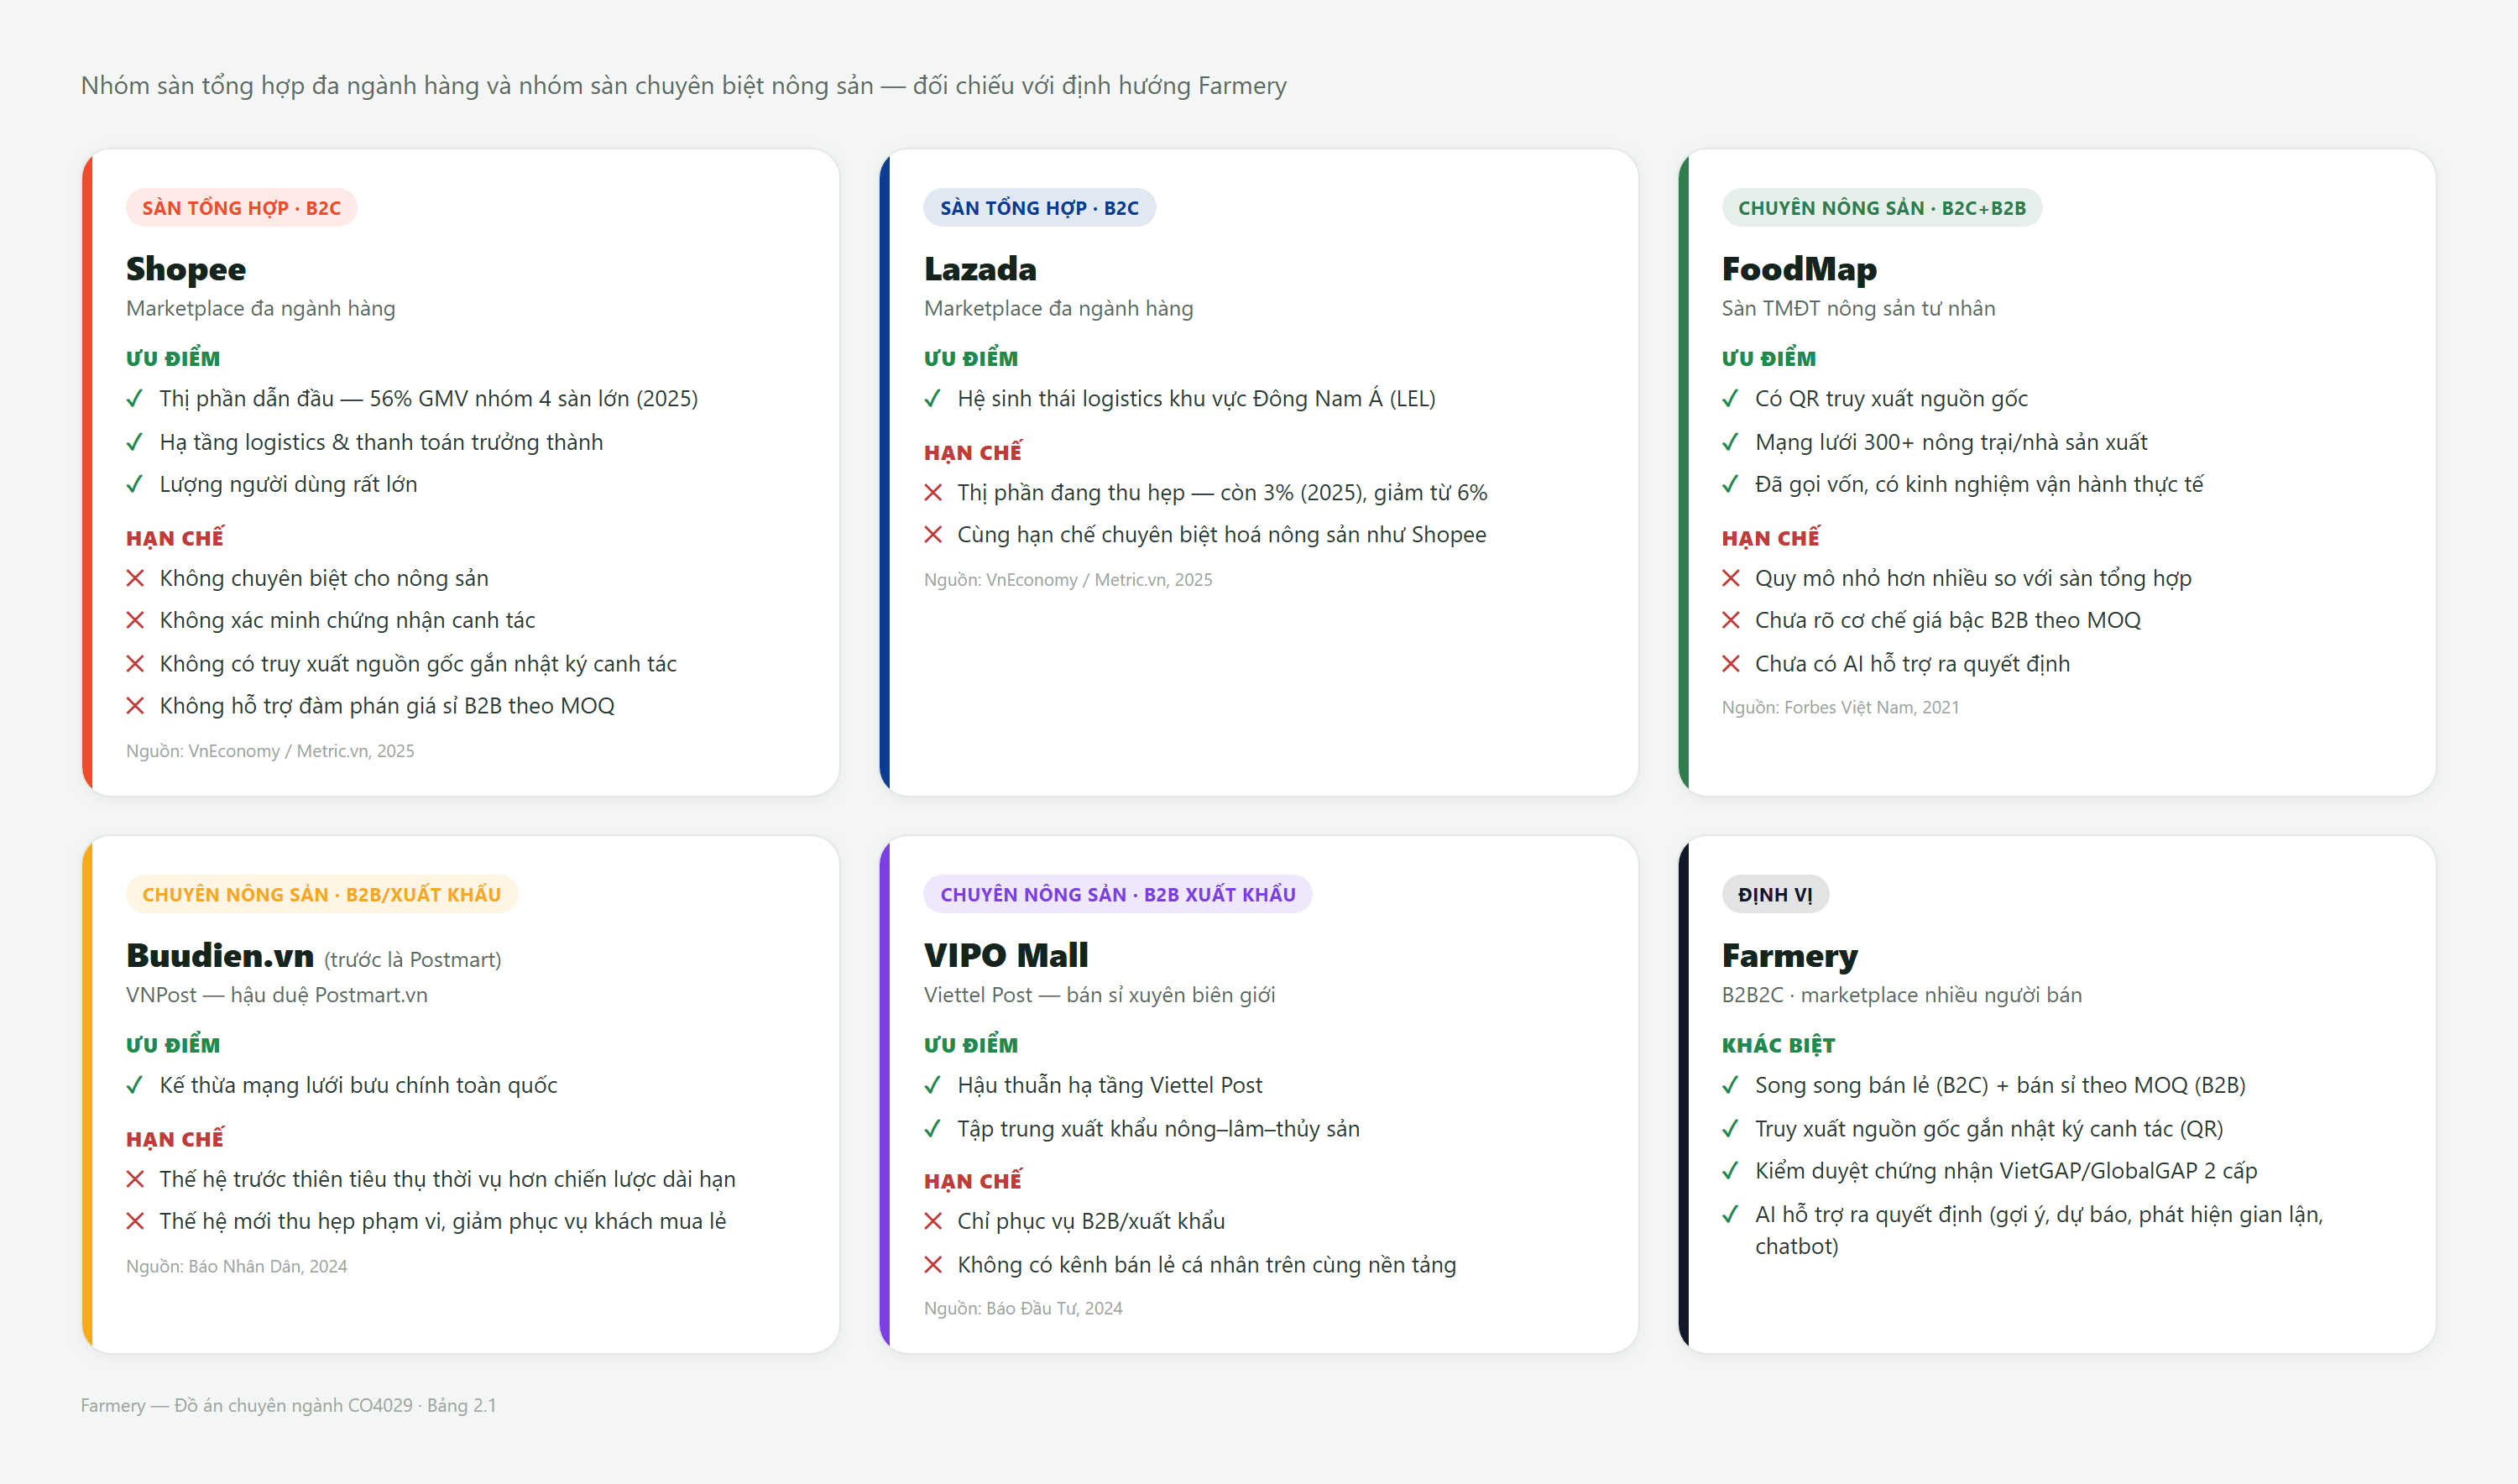
\includegraphics[width=\textwidth]{image/comparison/so-sanh-trong-nuoc.png}
\caption{So sánh các sàn thương mại điện tử trong nước liên quan đến nông sản}
\label{tab:sosanhtrongnuoc}
\end{figure}


\subsection{Các nền tảng quốc tế}
\label{subsec:sosanhquocte}

Ba nền tảng quốc tế dưới đây minh họa các hướng số hóa nông nghiệp khác nhau đã được kiểm chứng ở quy mô thương mại; Hình~\ref{tab:sosanhquocte} so sánh ưu/nhược điểm của chúng cùng với nghiên cứu Farm2Market đã trình bày tại mục~\ref{sec:nghiencuulienquan}:
\begin{itemize}
    \item \textbf{e-Choupal} (Ấn Độ, ITC, từ 2000) --- mô hình ``click and mortar'' dùng kiosk internet tại làng để loại bỏ tầng trung gian truyền thống (mandi/thương lái), giúp nông dân tăng thu nhập tới 50\% ở quy mô đã kiểm chứng (~4 triệu nông dân) \parencite{business_standard_2020_echoupal}.
    \item \textbf{Pinduoduo / Duo Duo Grocery} (Trung Quốc) --- mô hình mua chung (group buying) kết nối trực tiếp nông dân--người tiêu dùng, quy mô rất lớn (12 triệu+ nông dân, GMV nông nghiệp hàng trăm tỷ NDT) nhưng thuần B2C \parencite{nasdaq_2021_pinduoduo}.
    \item \textbf{Ninjacart} (Ấn Độ) --- nền tảng B2B rau củ tươi, dùng học máy dự báo nhu cầu và tối ưu vận chuyển, minh chứng AI có thể triển khai thực tế ở quy mô lớn cho hàng tươi, nhưng không phục vụ người tiêu dùng cá nhân \parencite{ninjacart}.
\end{itemize}

\begin{figure}[H]
\centering
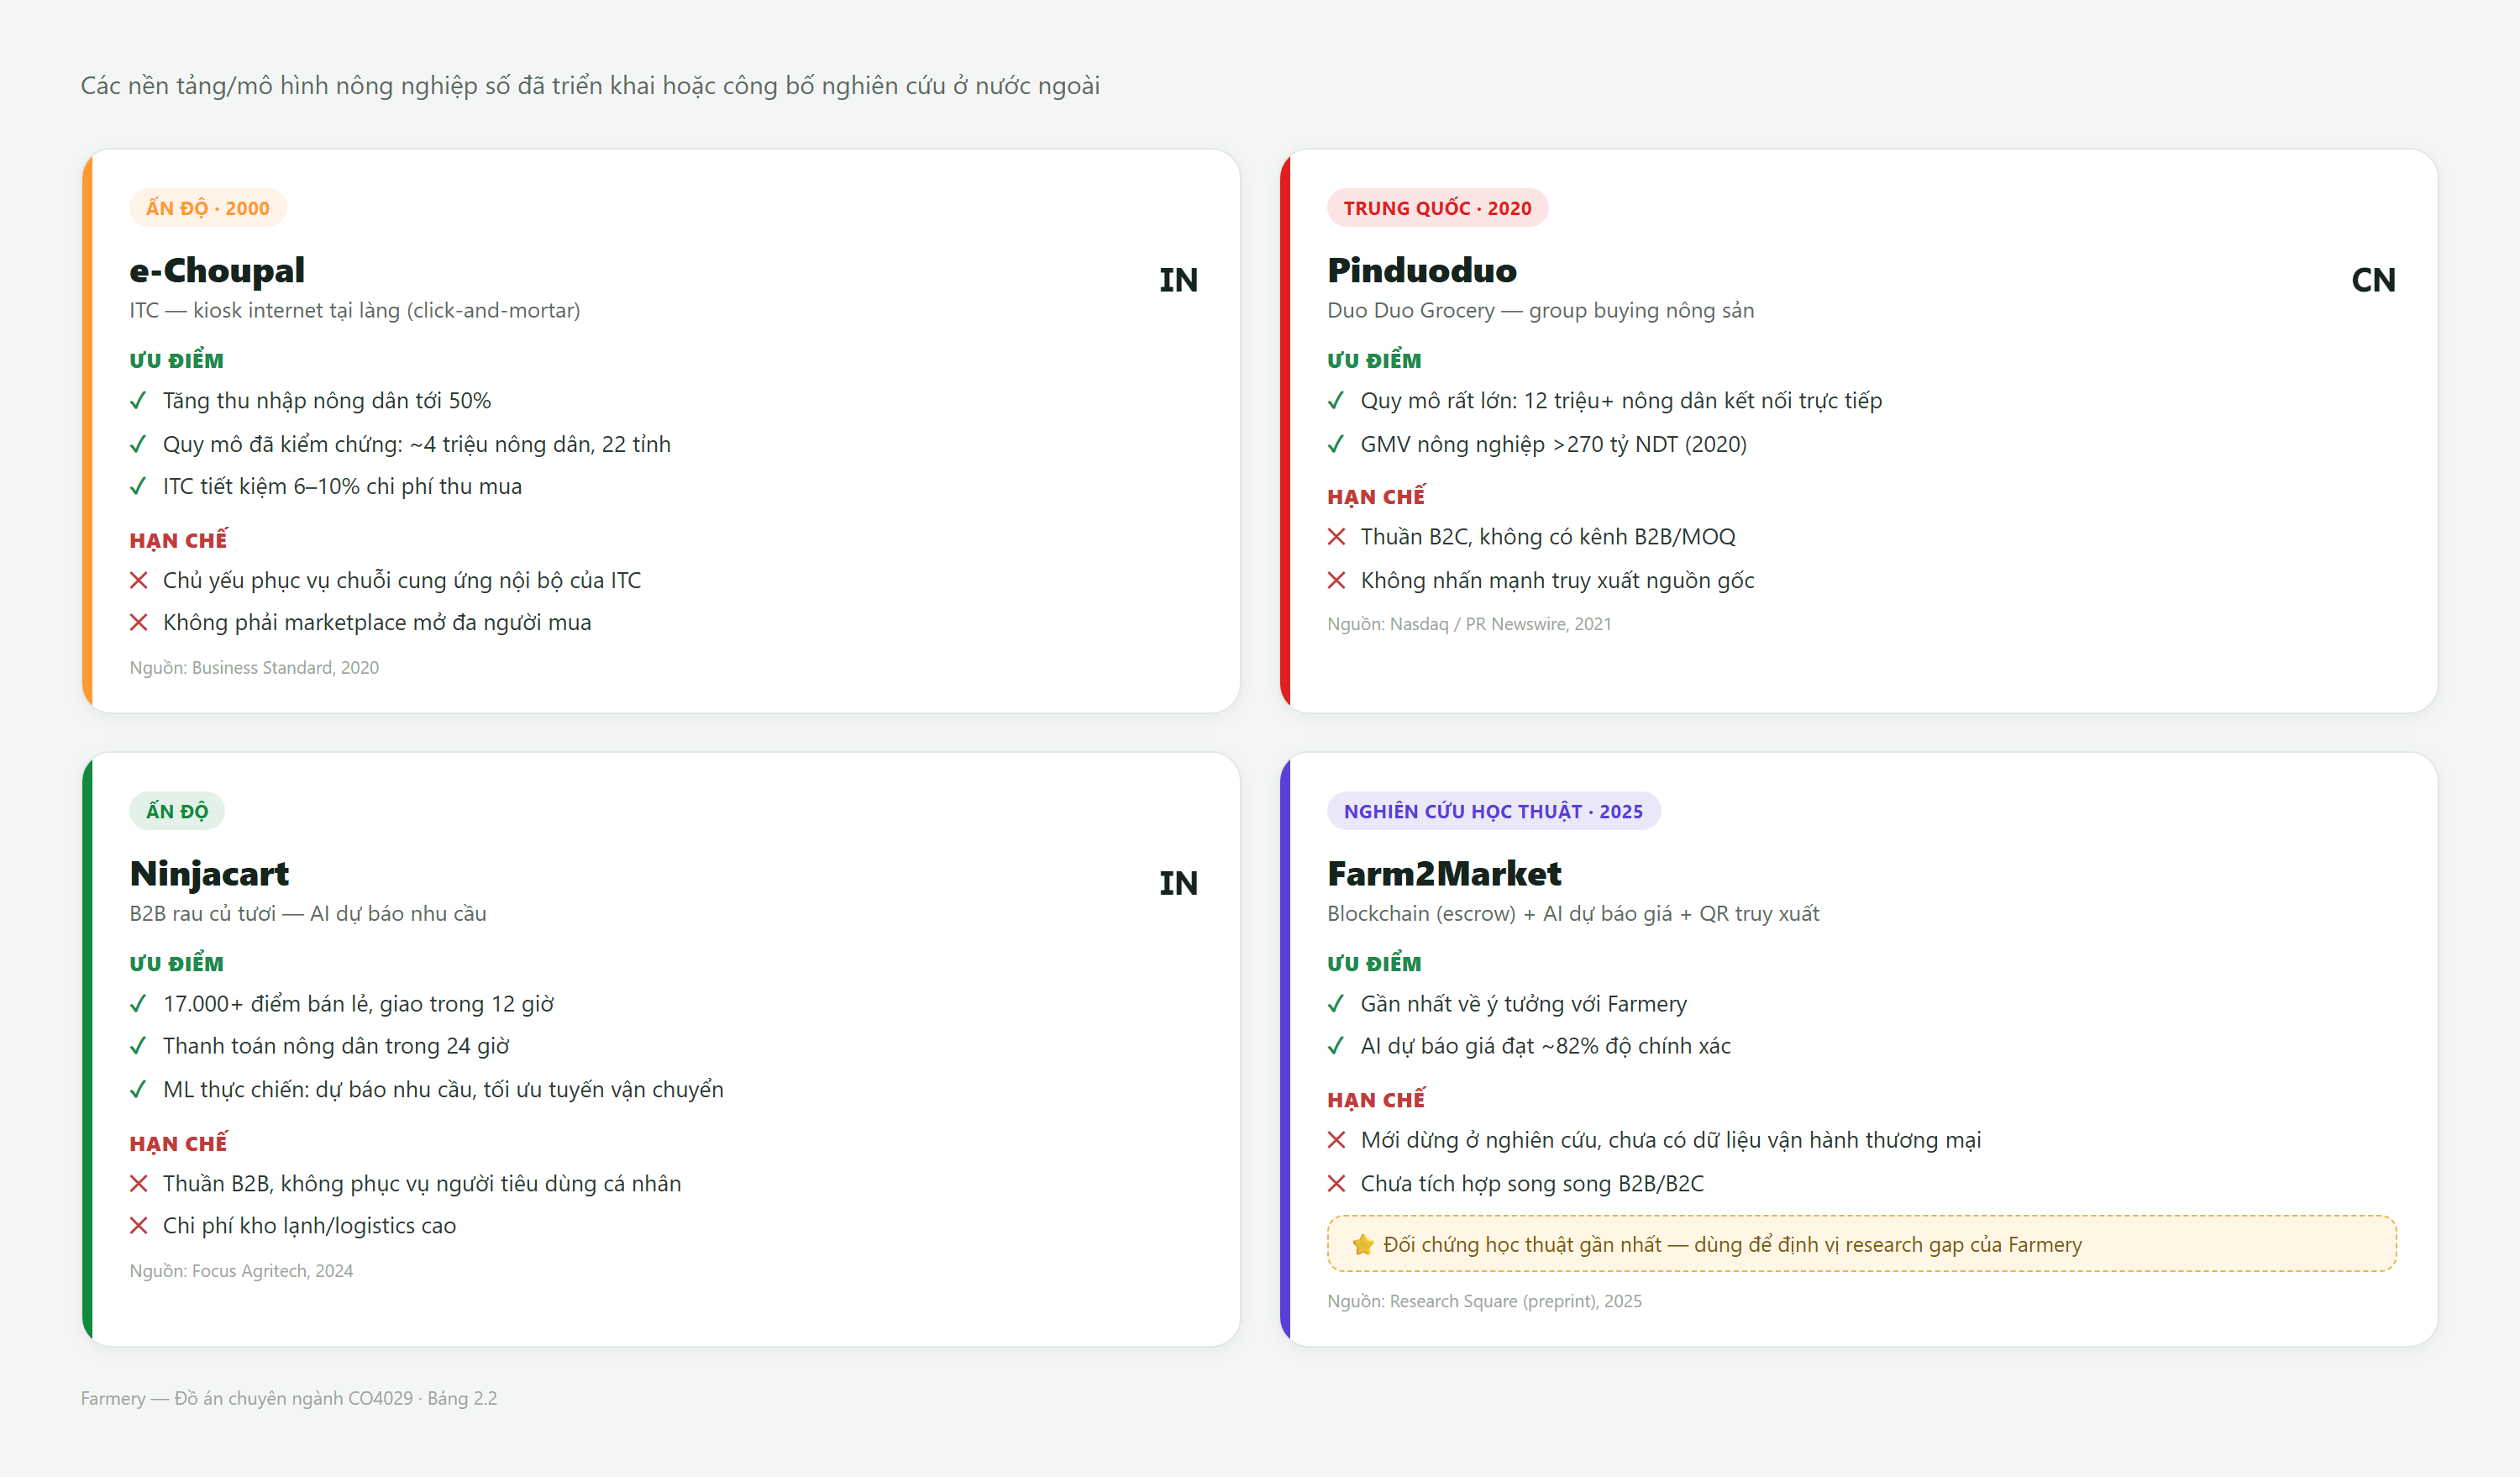
\includegraphics[width=\textwidth]{image/comparison/so-sanh-quoc-te.png}
\caption{So sánh các mô hình quốc tế tham khảo}
\label{tab:sosanhquocte}
\end{figure}


\section{Kết chương}
\label{subsec:researchgap}

Từ hai hình so sánh trên, có thể thấy phần lớn các nền tảng hiện có chỉ mạnh ở một phía --- hoặc thuần B2C (Pinduoduo, Shopee/Lazada đối với hàng nông sản), hoặc thuần B2B (Ninjacart, VIPO Mall, e-Choupal chủ yếu phục vụ chuỗi nội bộ) --- mà chưa tích hợp đầy đủ cả hai luồng bán lẻ và bán sỉ theo MOQ/giá bậc trên cùng một nền tảng. Tính năng truy xuất nguồn gốc bằng mã QR ở các sàn Việt Nam (FoodMap) hiện chủ yếu phục vụ minh bạch thông tin cơ bản, chưa gắn liền với nhật ký canh tác chi tiết theo chuẩn quốc tế (GS1 --- xem mục~\ref{subsec:gs1blockchain}). Farm2Market là mô hình gần nhất về mặt lý thuyết (kết hợp truy xuất nguồn gốc + AI + escrow) nhưng mới dừng ở nghiên cứu học thuật, chưa kiểm chứng ở quy mô vận hành thật, và không đề cập tới việc phục vụ song song hai luồng B2C/B2B. Hình~\ref{tab:researchgap} tổng hợp các tiêu chí này.

\begin{figure}[H]
\centering
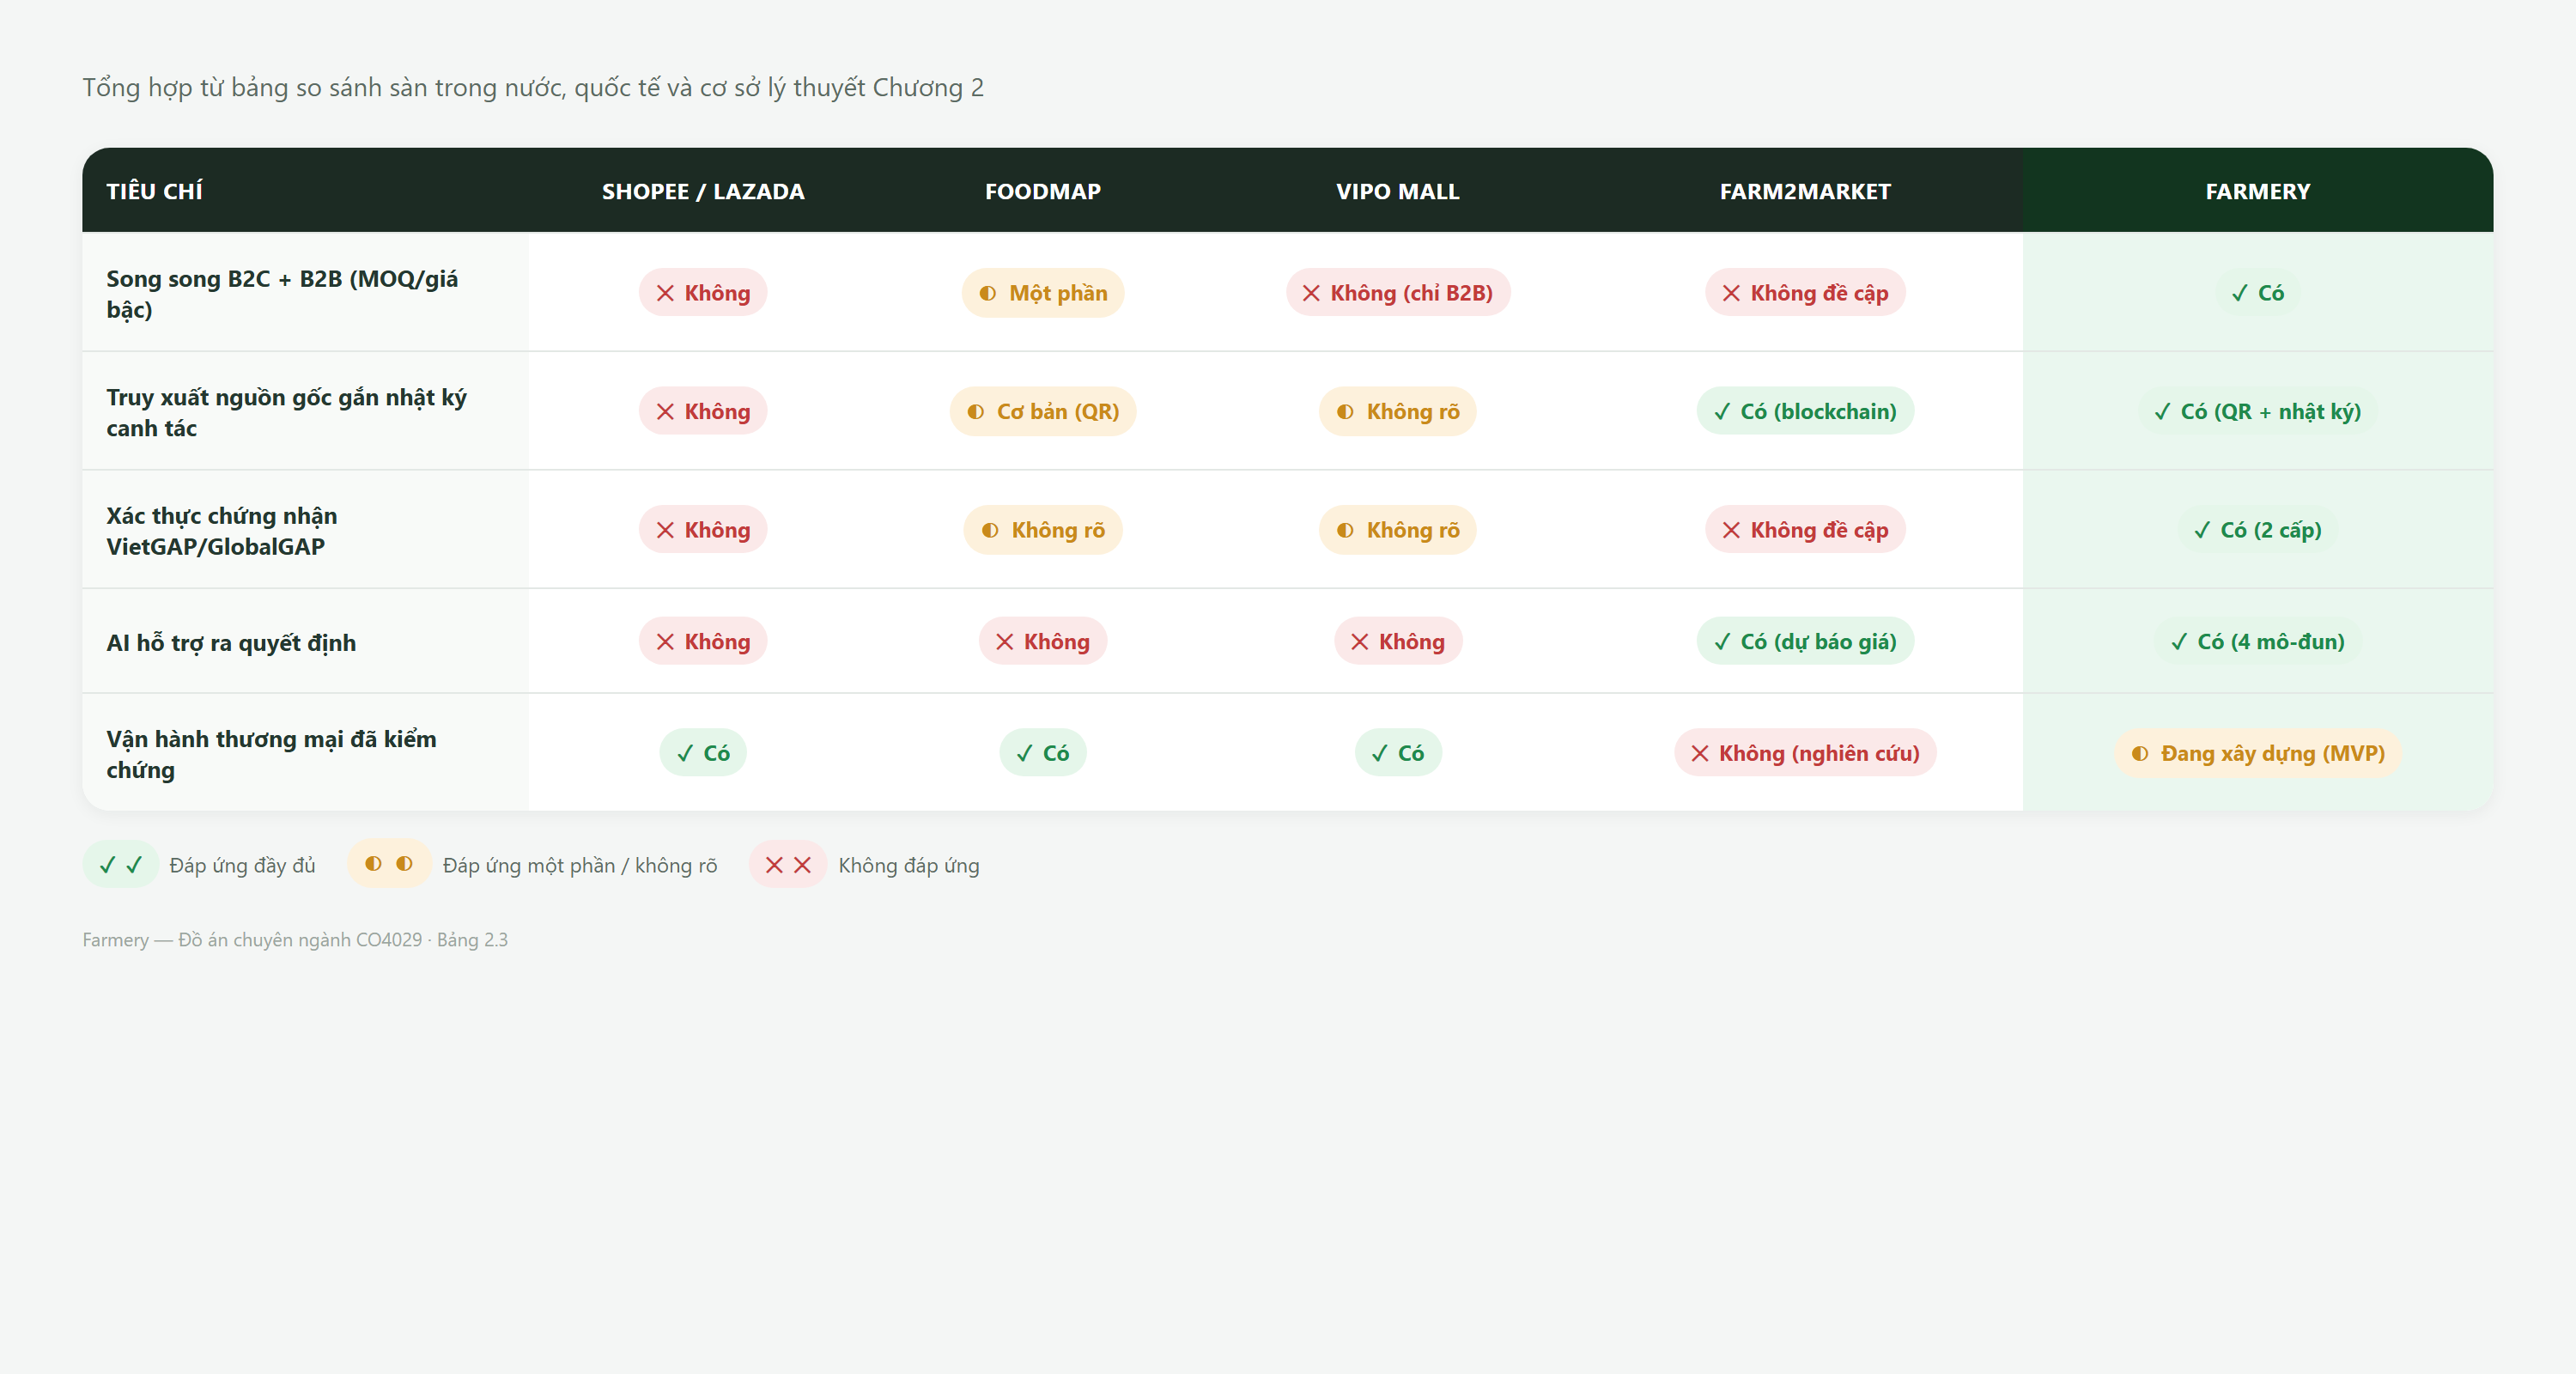
\includegraphics[width=\textwidth]{image/comparison/research-gap.png}
\caption{Ma trận khoảng trống nghiên cứu: Farmery so với các nền tảng đối chứng}
\label{tab:researchgap}
\end{figure}

Khoảng trống nghiên cứu mà Farmery hướng tới lấp đầy là: kết hợp truy xuất nguồn gốc gắn nhật ký canh tác theo nguyên lý GS1, hỗ trợ song song bán lẻ và bán sỉ B2B theo MOQ trên cùng một nền tảng, và tích hợp các mô-đun AI hỗ trợ ra quyết định (gợi ý sản phẩm, dự báo, phát hiện gian lận, trợ lý ảo) --- một tổ hợp chưa được các nền tảng đối chứng hiện thực hóa đầy đủ cùng lúc.

